
%%%%%%%%%%%%%%%%%%%%%%%%%%%%%%%%%%%%%%%%%%%%%%%%%%%%%%%%%%%%%%%%%%%%%%%%%%%%%%%%%%%%%%%
%%%%%%%%%%%%%%%%%%%%%%%%%%%%%%%%%%%%%%%%%%%%%%%%%%%%%%%%%%%%%%%%%%%%%%%%%%%%%%%%%%%%%%%
% 
% This top part of the document is called the 'preamble'.  Modify it with caution!
%
% The real document starts below where it says 'The main document starts here'.

\documentclass[12pt]{article}

\usepackage{amssymb,amsmath,amsthm}
\usepackage[top=1in, bottom=1in, left=1.25in, right=1.25in]{geometry}
\usepackage{fancyhdr}
\usepackage{enumerate}
\usepackage{listings}
\usepackage{graphicx}
\usepackage{float}

% Comment the following line to use TeX's default font of Computer Modern.
\usepackage{times,txfonts}



\makeatletter
\renewcommand*\env@matrix[1][*\c@MaxMatrixCols c]{%
  \hskip -\arraycolsep
  \let\@ifnextchar\new@ifnextchar
  \array{#1}}
\makeatother

\newtheoremstyle{homework}% name of the style to be used
  {18pt}% measure of space to leave above the theorem. E.g.: 3pt
  {12pt}% measure of space to leave below the theorem. E.g.: 3pt
  {}% name of font to use in the body of the theorem
  {}% measure of space to indent
  {\bfseries}% name of head font
  {:}% punctuation between head and body
  {2ex}% space after theorem head; " " = normal interword space
  {}% Manually specify head
\theoremstyle{homework} 

% Set up an Exercise environment and a Solution label.
\newtheorem*{exercisecore}{Exercise \@currentlabel}
\newenvironment{exercise}[1]
{\def\@currentlabel{#1}\exercisecore}
{\endexercisecore}

\newcommand{\localhead}[1]{\par\smallskip\noindent\textbf{#1}\nobreak\\}%
\newcommand\solution{\localhead{Solution:}}

%%%%%%%%%%%%%%%%%%%%%%%%%%%%%%%%%%%%%%%%%%%%%%%%%%%%%%%%%%%%%%%%%%%%%%%%
%
% Stuff for getting the name/document date/title across the header
\makeatletter
\RequirePackage{fancyhdr}
\pagestyle{fancy}
\fancyfoot[C]{\ifnum \value{page} > 1\relax\thepage\fi}
\fancyhead[L]{\ifx\@doclabel\@empty\else\@doclabel\fi}
\fancyhead[C]{\ifx\@docdate\@empty\else\@docdate\fi}
\fancyhead[R]{\ifx\@docauthor\@empty\else\@docauthor\fi}
\headheight 15pt

\def\doclabel#1{\gdef\@doclabel{#1}}
\doclabel{Use {\tt\textbackslash doclabel\{MY LABEL\}}.}
\def\docdate#1{\gdef\@docdate{#1}}
\docdate{Use {\tt\textbackslash docdate\{MY DATE\}}.}
\def\docauthor#1{\gdef\@docauthor{#1}}
\docauthor{Use {\tt\textbackslash docauthor\{MY NAME\}}.}
\makeatother

% Shortcuts for blackboard bold number sets (reals, integers, etc.)
\newcommand{\Reals}{\ensuremath{\mathbb R}}
\newcommand{\Nats}{\ensuremath{\mathbb N}}
\newcommand{\Ints}{\ensuremath{\mathbb Z}}
\newcommand{\Rats}{\ensuremath{\mathbb Q}}
\newcommand{\Cplx}{\ensuremath{\mathbb C}}
%% Some equivalents that some people may prefer.
\let\RR\Reals
\let\NN\Nats
\let\II\Ints
\let\CC\Cplx

%%%%%%%%%%%%%%%%%%%%%%%%%%%%%%%%%%%%%%%%%%%%%%%%%%%%%%%%%%%%%%%%%%%%%%%%%%%%%%%%%%%%%%%
%%%%%%%%%%%%%%%%%%%%%%%%%%%%%%%%%%%%%%%%%%%%%%%%%%%%%%%%%%%%%%%%%%%%%%%%%%%%%%%%%%%%%%%
% 
% The main document start here.

% The following commands set up the material that appears in the header.
\doclabel{STAT 401: Homework 3}
\docauthor{Stefano Fochesatto}
\docdate{\today}


%\begin{figure}[H]
%  \begin{center}
%  \caption{}
%  \includegraphics[\textwidth]{}
%  \end{center}
%\end{figure}

% \textbf{Code:}
% \begin{center}
% \lstinputlisting{}
% \end{center} 



\begin{document}

\begin{exercise}{1} Do Problem 2.6. Skip 2.6.4\\
  The data file give the mean temperatures in the fall of each year, 
  defined as September 1 to November 30 and the mean temperature in the following
  winter, defined as December 1 to the end of February in the following calender year\dots
  These data cover the time period from 1900 to 2010. the question of interest is: Does the 
  average fall temperature predict the average winter temperature. 
  \begin{enumerate}
    \item Draw a scatter plot of the response versus the predictor, and describe any pattern 
    you might see.
    \solution 
    \begin{figure}[H]
      \begin{center}
      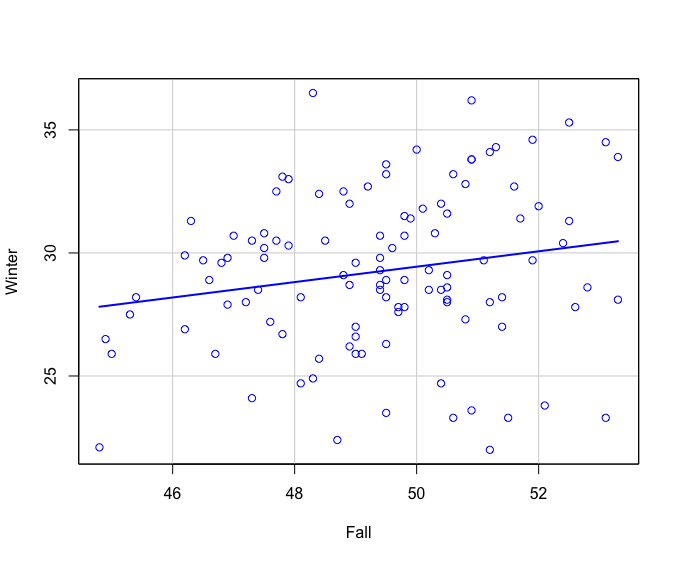
\includegraphics[width = .75 \textwidth]{Rplot.png}
      \end{center}
    \end{figure}
        \textbf{Code:}
        \begin{center}
        \lstinputlisting{r1.txt}
        \end{center} 
        It is difficult to infer from a simple scatter plot, the relationship between 
        both variables. There does seem to be a grouping in the center with a slightly positive 
        relationship. 
        \newpage

    \item Use statistical software to fit the regression of the response on the
    predictor. Add the fitted line to you graph(done in previous figure). Test the slope to be 0 against 
    a two-sided alternative, and summarize your results.\\
    \solution
    The following, describes a SLR for the response on the predictor. \\
    \textbf{Code:}
        \begin{center}
        \lstinputlisting{r2.txt}
        \end{center} 
    
    Stating our hypothesis, If there is a significant linear relationship between 
    the fall temperature and the winter temperature, 
    the slope will not equal zero. Defining our experiment, 
    \begin{equation*}
      H_0: \beta_1 = 0
    \end{equation*}
    \begin{equation*}
      H_A: \beta_1 \neq 0
    \end{equation*}
    Computing the test statistic, 
    \begin{equation*}
      t = \dfrac{\hat{\beta}_1}{S.E(\hat{\beta}_1)} = \dfrac{0.3132}{0.1528} = 2.04973
    \end{equation*}
    Evaluating the p-value for a t-distribution on 109 df we get $p = 0.04279$. On the $\alpha = .05$
    significance level we get that there is a statistically significant relationship between 
    the fall and winter temperatures. 
    \newpage

    \item Compute or obtain from your computer output, the value of the variability 
    in winter explained by fall and explain what this means. \\
    \solution The variability in winter explained by the linear regression on 
    the fall data is the sum of squares for regression(SSreg) and the $R^2$ value gives us 
    that as a percentage of the total variability,
    \begin{equation*}
      R^2 = \dfrac{SSreg}{SSreg+RSS}  =  \dfrac{SSreg}{SYY} = \dfrac{42.446}{42.446 + 1101.69} = 0.0371021
    \end{equation*}
    What this means is our model explains $~3.7\%$ of the variability in response variable. 
    We can compute these values using anova(), summary(lm()) or by-hand with r. 
    \textbf{Code:}
        \begin{center}
        \lstinputlisting{r3.txt}
        \end{center} 
  \end{enumerate}
\end{exercise}
\newpage

\begin{exercise}{2} For the data set in problem 2.6, do the following.
  \begin{enumerate}
    \item Calculate a $95\%$ confidence interval for the model intercept.\\
    \solution We compute the $95\%$ confidence interval for the model intercept
    using the following formula, 
    \begin{equation*}
      \hat{\beta}_0 \pm t_{.05}\hat{\sigma}\left(\dfrac{1}{n} \dfrac{\bar{x}^2}{SXX}\right)
    \end{equation*}
    We can also compute it using r, with the following,\\
    \textbf{Code:}
    \begin{center}
    \lstinputlisting{r4.txt}
    \end{center} 
    \newpage

    \item Produce an effect plot for the effect of fall on the mean of winter. \\
    \solution
    \begin{figure}[H]
      \begin{center}
      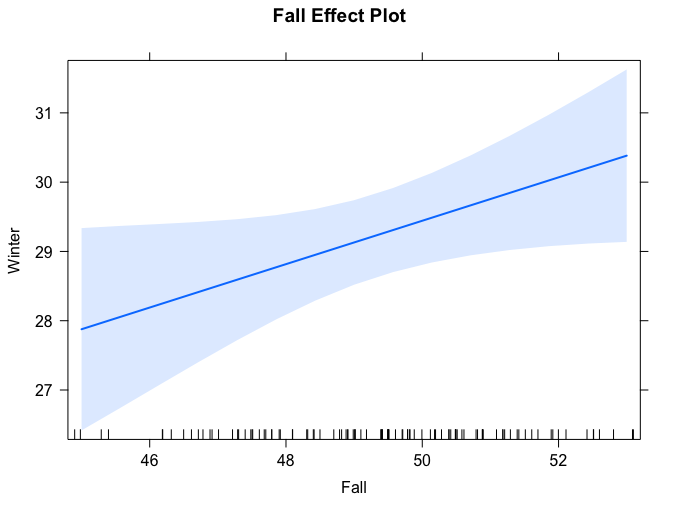
\includegraphics[width = .75 \textwidth]{Rplot02.png}
      \end{center}
    \end{figure}
        \textbf{Code:}
        \begin{center}
        \lstinputlisting{r5.txt}
        \end{center}
    \newpage

    \item What are the values for the smallest and largest residuals. \\
    \solution
    \textbf{Code:}
    \begin{center}
    \lstinputlisting{r6.txt}
    \end{center}
    \newpage

    \item Interpret the residual plot shown below in terms of the appropriateness
    of the linear model.
    \begin{figure}[H]
      \begin{center}
      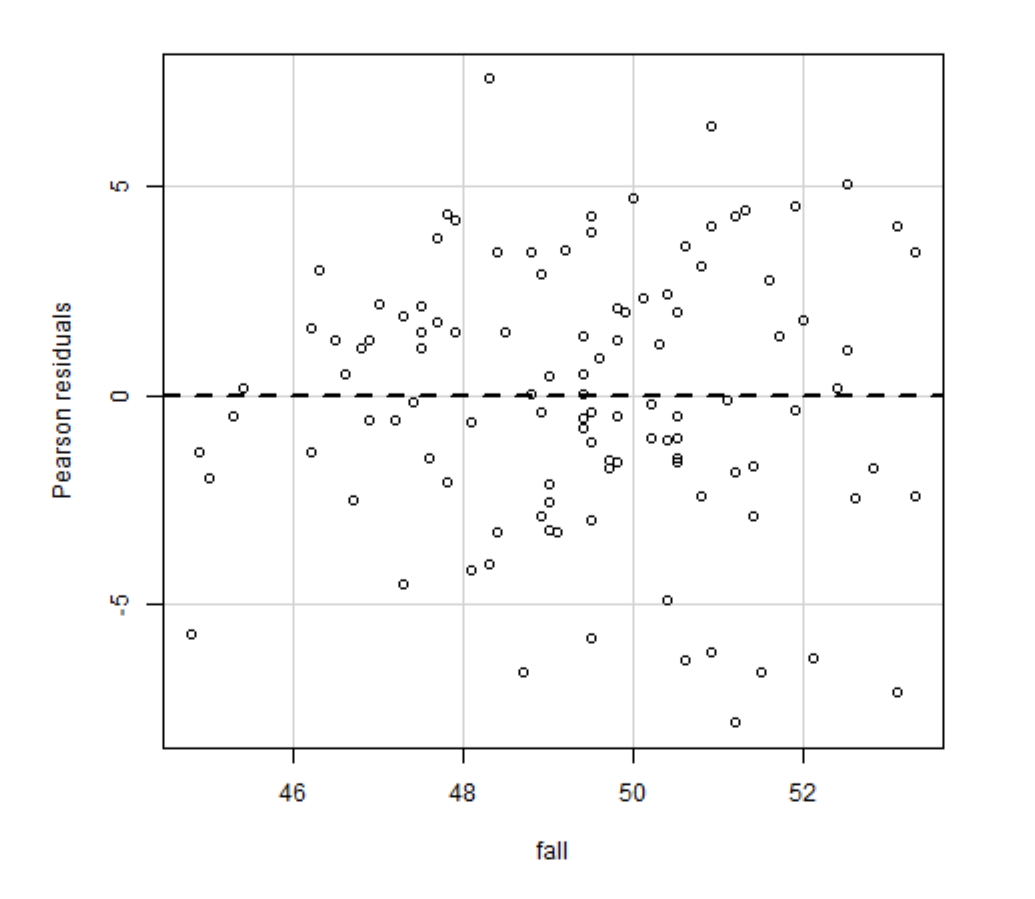
\includegraphics[width = .75 \textwidth]{Rplot03.png}
      \end{center}
    \end{figure}
    \solution The residual plot shows no obvious clustering or patterns which would
    suggest that our model is an appropriate fit.
  \end{enumerate}
\end{exercise}
\newpage

\begin{exercise}{2.13} Heights of mothers and daughters.
  \begin{enumerate}
    \item Compute the regression of $dheight$ on $mheight$, and report the estimates,
    their standard errors, the value of the coefficient of determination, and the estimate of 
    variance. Write a sentence or two that summarizes the results of these computations.\\
    \solution Using r, we can fit the regression we get the following, \\
    \textbf{Code:}
    \begin{center}
    \lstinputlisting{r7.txt}
    \end{center}
    Interpreting the linear model, we can say that for every one inch a mother's height increases
    we can expect her daughter's to increase by approximately .5 inches. The standard errors give us a good
    idea of were the true regression parameters may be. An $R^2$ value of .2406 suggests that our model 
    doesn't do an excellent job of explaining all the variance in the data. 
    \newpage

    \item Obtain a $99\%$ confidence interval for $\beta_1$ from the data.\\
    \solution 
    \textbf{Code:}
    \begin{center}
    \lstinputlisting{r8.txt}
    \end{center}
    \newpage

    \item Obtain a prediction and $99\%$ prediction interval for a daughter 
    whose mother is 64 inches tall.\\
    \solution
    \textbf{Code:}
    \begin{center}
    \lstinputlisting{r9.txt}
    \end{center}
  \end{enumerate}
\end{exercise}
\newpage


\begin{exercise}{4} For the data set in problem 2.13, do the following.
  \begin{enumerate}
    \item Calculate the value of the correlation coefficient $r$
    \solution Recall that, 
    \begin{equation*}
      r = \dfrac{SXY}{\sqrt{SXX*SYY}} = \sqrt{R^2}
    \end{equation*}
    We can compute each term and use the formula or we can just square root the 
    value given in the summary of the linear model.\\
    \textbf{Code:}
    \begin{center}
    \lstinputlisting{r10.txt}
    \end{center}
    \newpage

    \item If the intercept-only model is fit to the data, what is it's estimated intercept 
    $\hat{\beta}_0$?\\
    \solution The intercept only model is computed by finding the mean of the response variables.
    Here is an interesting way of computing it using the lm() command, \\
    \textbf{Code:}
    \begin{center}
    \lstinputlisting{r11.txt}
    \end{center}
    \newpage

    \item Produce the Anova table for this model. Be sure to include a "Total" row in your table. \\
    \solution
    \textbf{Code:}
    \begin{center}
    \lstinputlisting{r12.txt}
    \end{center}
    \newpage

    \item If the predictor $mheight$ is standardized before fitting the model, the resulting fitted 
    model becomes $E(Y) = 63.75 + .54x$. Interpret the slope and intercept in this model.\\
    \solution Since the slope is unchanged from the previous fitting I will assume that the method of standardizing
    was just centering. When you center your predictor variable, you just subtract the mean from every data. This makes so
    that the intercept becomes the predicted value for the mean predictor. So for average height women, their daughters are expected to 
    be around $63.75$. The slope continues to have the same interpretation as before. 
  \end{enumerate}
  
\end{exercise}

\end{document}





















